\documentclass[12pt]{article}
\usepackage[utf8]{inputenc}
\usepackage[T1]{fontenc}
\usepackage{amsmath, amssymb, amsfonts}
\usepackage{geometry}
\geometry{a4paper, margin=1in}
\usepackage{hyperref}
\usepackage{tcolorbox}
\usepackage{graphicx}
\usepackage{enumitem}
\usepackage{pgfplots}
\pgfplotsset{compat=1.18}

% Custom environments for the blocks found in the text
\newtcolorbox{definitionbox}[1][]{colback=blue!5!white,colframe=blue!75!black,title=\textbf{Definition},#1}
\newtcolorbox{keyresultbox}[1][]{colback=green!5!white,colframe=green!75!black,title=\textbf{Key Result},#1}
\newtcolorbox{insightbox}[1][]{colback=orange!5!white,colframe=orange!75!black,title=\textbf{Practical Insight},#1}
\newtcolorbox{pitfallbox}[1][]{colback=red!5!white,colframe=red!75!black,title=\textbf{Pitfall / Caution},#1}

\title{Implied Volatility and Volatility Surfaces \\ \large A Comprehensive Course Note}
\author{Karim Khodjerane}
\date{December 23, 2025}

\begin{document}

\maketitle

\begin{abstract}
\noindent Focus: equity/FX-style volatility quoting, smiles/skews, surface construction, no-arbitrage constraints, and links to local volatility and risk-neutral density.
\end{abstract}

\tableofcontents

\newpage

\section{Notation and Setup}

We work under a frictionless market with deterministic interest rate $r$ (for simplicity) and a non-dividend-paying underlying $S_t$ unless stated otherwise. Let $T$ be maturity, $K$ strike, and $\tau = T - t$ time-to-maturity.

\begin{definitionbox}
\textbf{Forward price.} For maturity $T$, the (time-$t$) forward is
\[ F_{t,T} = S_t e^{(r-q)\tau}, \]
where $q$ is the continuous dividend yield (or foreign rate in FX). In what follows, we often use $F$ as the natural reference level for moneyness.
\end{definitionbox}

\begin{definitionbox}
\textbf{Discount factor.} With deterministic $r$, the discount factor is
\[ D(t, T) = e^{-r\tau}. \]
\end{definitionbox}

\section{Black--Scholes Price and the Definition of Implied Volatility}

\subsection{Black--Scholes call/put formulas}

Under the Black--Scholes model with constant volatility $\sigma$, the time-$t$ price of a European call is
\[ C_{BS}(t; S_t, K, T, \sigma) = D(t, T) [ F_{t,T} \Phi(d_1) - K \Phi(d_2) ], \]
and the put is
\[ P_{BS}(t; S_t, K, T, \sigma) = D(t, T) [ K \Phi(-d_2) - F_{t,T} \Phi(-d_1) ], \]
where
\[ d_1 = \frac{\ln(F_{t,T}/K) + \frac{1}{2}\sigma^2\tau}{\sigma\sqrt{\tau}}, \quad d_2 = d_1 - \sigma\sqrt{\tau}, \]
and $\Phi$ is the standard normal CDF.

\begin{keyresultbox}
\textbf{Put--call parity (forward form).}
\[ C - P = D(t, T) (F_{t,T} - K). \]
This relation is model-free (no-arbitrage).
\end{keyresultbox}

\subsection{Implied volatility}

Market option prices are rarely consistent with a constant volatility. Instead, practitioners quote options by the volatility $\sigma$ that makes the Black--Scholes price match the observed market price.

\begin{definitionbox}
\textbf{Implied volatility.} Given an observed market price $C_{mkt}$ for a European call, the implied volatility $\sigma_{imp}$ is the (unique) solution to
\[ C_{BS}(t; S_t, K, T, \sigma_{imp}) = C_{mkt}. \]
Similarly for a put.
\end{definitionbox}

\begin{insightbox}
Implied volatility is a re-parameterization of option prices. It is not the true future realized volatility. It is the volatility that, plugged into Black--Scholes, reproduces the market price.
\end{insightbox}

\section{Existence, Uniqueness, and Numerical Computation}

\subsection{Why the implied volatility exists (in practice)}

For standard European options, the Black--Scholes price is increasing in $\sigma$ (positive Vega), so inversion is well-posed.

\begin{keyresultbox}
\textbf{Vega (sensitivity to volatility).} For a call or put in Black--Scholes:
\[ \mathcal{V} = \frac{\partial C_{BS}}{\partial \sigma} = D(t, T) F_{t,T} \phi(d_1) \sqrt{\tau} > 0, \]
where $\phi$ is the standard normal PDF. Therefore $C_{BS}(\sigma)$ is strictly increasing in $\sigma$.
\end{keyresultbox}

\begin{pitfallbox}
In practice, data issues can break inversion:
\begin{itemize}
    \item stale quotes,
    \item bid--ask noise,
    \item violations of static arbitrage (e.g., call price decreasing in $K$),
    \item too deep OTM quotes with tiny prices (numerical instability).
\end{itemize}
Always clean quotes before building a surface.
\end{pitfallbox}

\subsection{How we compute implied volatility}

Closed-form inversion does not exist for Black--Scholes. We solve a 1D root-finding problem:
\[ f(\sigma) = C_{BS}(\sigma) - C_{mkt} = 0. \]

\begin{insightbox}
\textbf{Standard methods.}
\begin{itemize}
    \item Newton--Raphson: fast, uses Vega.
    \item Bisection: slow but robust (guaranteed convergence if bracketing).
    \item Hybrid methods: bisection + Newton for stability.
\end{itemize}
A good initial guess matters, especially for short maturities or extreme strikes.
\end{insightbox}

\section{Moneyness, Log-Moneyness, and Volatility Quotes}

\subsection{Choice of x-axis: strike vs moneyness}

Option smiles are clearer when plotted against moneyness.

\begin{definitionbox}
\textbf{Log-moneyness (forward).}
\[ k = \ln \left( \frac{K}{F_{t,T}} \right). \]
ATM-forward corresponds to $k = 0$.
\end{definitionbox}

\begin{insightbox}
Why forward-moneyness is preferred:
\begin{itemize}
    \item it removes the drift/discounting effect,
    \item it makes smiles more comparable across maturities,
    \item it matches the risk-neutral measure naturally used in pricing.
\end{itemize}
\end{insightbox}

\subsection{Delta conventions (especially FX)}

In FX, quotes often come in delta space rather than strike space. You convert between delta and strike using the Black--Scholes formulas plus the chosen delta convention (spot delta, forward delta, premium-adjusted delta, etc.).

\begin{pitfallbox}
Delta-to-strike conversion depends on:
\begin{itemize}
    \item call/put,
    \item spot vs forward delta,
    \item whether delta is premium-adjusted,
    \item domestic/foreign discounting.
\end{itemize}
Always document the market convention used.
\end{pitfallbox}

\section{Volatility Smile and Skew: Shapes and Intuition}

\subsection{What is a smile?}

A volatility smile means implied volatility varies with strike:
\[ \sigma_{imp} = \sigma_{imp}(K, T). \]

Typically, equity indices show a \textbf{left skew}: high implied vols for low strikes (crash protection is expensive).

\begin{definitionbox}
\textbf{Smile vs skew.}
\begin{itemize}
    \item \textbf{Smile:} U-shaped curve vs $K$ or $k$.
    \item \textbf{Skew:} monotone slope, often stronger on one side (equity downside).
\end{itemize}
\end{definitionbox}

\subsection{Economic interpretation (qualitative)}

\begin{insightbox}
Common drivers behind smile/skew (intuition):
\begin{itemize}
    \item \textbf{Fat tails and non-normal returns} under the pricing measure.
    \item \textbf{Leverage effect}: volatility rises when the underlying falls (equities).
    \item \textbf{Jumps}: discontinuous moves produce pronounced smiles.
    \item \textbf{Supply/demand}: persistent demand for puts lifts downside implied vols.
\end{itemize}
Implied volatility reflects both probabilistic beliefs and risk premia.
\end{insightbox}

\subsection{Illustration: a typical equity skew}

% Placeholder for illustration
\begin{center}
    \fbox{\parbox{0.8\textwidth}{\centering \vspace{1cm} [Illustration: Plot of Implied volatility vs Log-moneyness $k$, showing a skew (higher for $k<0$)] \vspace{1cm}}}
\end{center}

\section{Term Structure of Implied Volatility}

Implied volatility changes with maturity. For short maturities, microstructure and jump risk matter more. For long maturities, mean reversion and macro uncertainty dominate.

\begin{definitionbox}
\textbf{Term structure.} Fix a strike (or moneyness) and view implied vol as a function of maturity:
\[ T \mapsto \sigma_{imp}(K, T). \]
\end{definitionbox}

\begin{insightbox}
Typical patterns:
\begin{itemize}
    \item \textbf{Event-driven hump}: elevated short maturities around earnings/meetings.
    \item \textbf{Downward short-end}: if near-term uncertainty is low.
    \item \textbf{Upward long-end}: if long-run uncertainty dominates.
\end{itemize}
\end{insightbox}

\section{From Smile to Volatility Surface}

\subsection{Definition of a volatility surface}

\begin{definitionbox}
\textbf{Volatility surface.} A volatility surface is a function
\[ (K, T) \mapsto \sigma_{imp}(K, T), \]
(or equivalently $(k, T) \mapsto \sigma_{imp}(k, T)$) built from market quotes across strikes and maturities.
\end{definitionbox}

\subsection{Visual illustration: a stylized surface}

% Placeholder for illustration
\begin{center}
    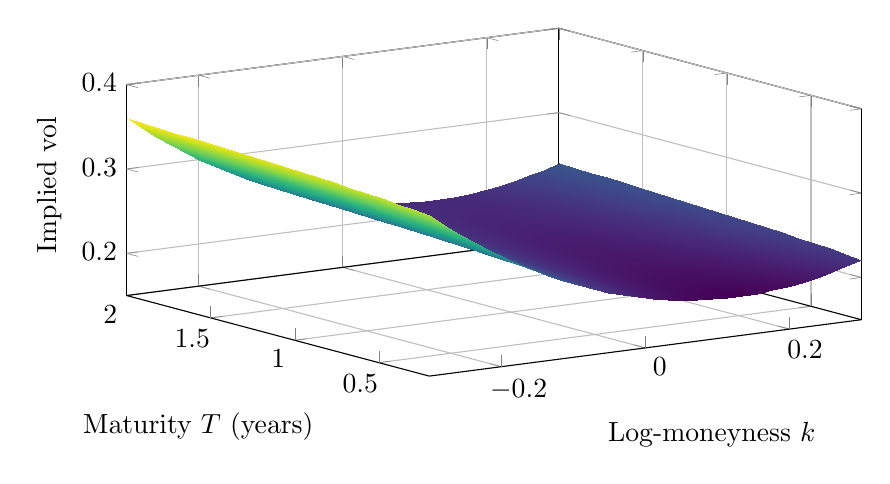
\begin{tikzpicture}
        \begin{axis}[
            width=0.9\textwidth,
            height=6cm,
            view={-35}{25}, % Adjust view angle
            xlabel={Log-moneyness $k$},
            ylabel={Maturity $T$ (years)},
            zlabel={Implied vol},
            zlabel style={},
            colormap/viridis,
            shader=interp,
            grid=major,
            title={},
            xmin=-0.3, xmax=0.3,
            ymin=0.2, ymax=2.0,
            zmin=0.15, zmax=0.4
        ]
        \addplot3[
            surf,
            domain=-0.3:0.3,
            domain y=0.2:2.0,
            samples=30,
            samples y=20,
        ]
        {0.2 + 0.8*x^2 - 0.2*x + 0.02*sqrt(y)}; % A stylized volatility surface with skew and term structure
        \end{axis}
    \end{tikzpicture}
\end{center}

\begin{insightbox}
Reading the surface:
\begin{itemize}
    \item Fix $T$: you see a smile/skew slice.
    \item Fix $k$: you see the term structure.
    \item Equity surfaces: downside skew is often strongest at short maturities and gradually flattens.
\end{itemize}
\end{insightbox}

\section{Static No-Arbitrage Constraints for Surfaces}

A volatility surface is only useful if it corresponds to a set of option prices that does not violate static arbitrage.

\subsection{No-arbitrage in strike (butterfly arbitrage)}

For a fixed maturity $T$, call prices as a function of strike must satisfy:
\[ \frac{\partial C}{\partial K} \leq 0, \quad \frac{\partial^2 C}{\partial K^2} \geq 0. \]
The second condition is convexity and prevents butterfly arbitrage.

\begin{keyresultbox}
\textbf{Risk-neutral density (Breeden--Litzenberger).} Under mild regularity,
\[ \frac{\partial^2 C}{\partial K^2} = D(t, T) f_{S_T}(K), \]
where $f_{S_T}(K)$ is the risk-neutral density of $S_T$. Hence convexity ($\partial^2 C / \partial K^2 \geq 0$) is equivalent to a nonnegative density.
\end{keyresultbox}

\subsection{No-arbitrage across maturities (calendar arbitrage)}

For a fixed strike $K$, call prices must be non-decreasing with maturity:
\[ C(K, T_2) \geq C(K, T_1) \quad \text{if } T_2 > T_1. \]

\begin{pitfallbox}
A surface may look smooth in implied-vol space but still violate arbitrage in price space. \textbf{Always check constraints in price space}, not only in volatility space.
\end{pitfallbox}

\section{Building a Volatility Surface in Practice}

\subsection{Step-by-step workflow}

\begin{insightbox}
\textbf{Pipeline (standard desk approach).}
\begin{enumerate}
    \item Collect quotes (bid/ask) for several maturities and strikes or deltas.
    \item Convert everything to a consistent convention:
    \begin{itemize}
        \item use forward $F_{t,T}$,
        \item map delta-quotes to strikes if needed,
        \item choose call/put consistently and enforce put--call parity.
    \end{itemize}
    \item Clean data:
    \begin{itemize}
        \item remove obvious outliers,
        \item ensure monotonicity/convexity (or regularize).
    \end{itemize}
    \item Fit each maturity slice (smile fit):
    \begin{itemize}
        \item parametric (SVI, polynomial on $k$ with constraints, etc.),
        \item or nonparametric (splines with arbitrage control).
    \end{itemize}
    \item Interpolate across maturities:
    \begin{itemize}
        \item interpolate total variance $w(k, T) = \sigma_{imp}^2(k, T) T$ rather than $\sigma$,
        \item enforce calendar constraints.
    \end{itemize}
    \item Validate:
    \begin{itemize}
        \item reproduce market quotes within bid/ask,
        \item run arbitrage checks,
        \item stress-test stability.
    \end{itemize}
\end{enumerate}
\end{insightbox}

\subsection{Why interpolate total variance?}

\begin{definitionbox}
\textbf{Total implied variance.}
\[ w(k, T) = \sigma_{imp}^2(k, T) T. \]
\end{definitionbox}

\begin{insightbox}
Interpolating $w$ is often more stable because:
\begin{itemize}
    \item it behaves more linearly in $T$,
    \item it aligns with diffusion scaling,
    \item it helps enforce calendar monotonicity ($w$ typically increases with $T$).
\end{itemize}
\end{insightbox}

\section{A Standard Parametric Smile: SVI (Overview)}

\subsection{SVI idea}

A popular model to fit a single maturity slice is SVI (Stochastic Volatility Inspired). It parameterizes total variance as a function of log-moneyness.

\begin{definitionbox}
\textbf{SVI total variance (one common form).}
\[ w(k) = a + b \left[ \rho(k-m) + \sqrt{(k-m)^2 + \sigma^2} \right], \]
with parameters $a, b, \rho, m, \sigma$.
\end{definitionbox}

\begin{insightbox}
SVI is used because it:
\begin{itemize}
    \item fits many market smiles well,
    \item is flexible yet compact,
    \item can be constrained to reduce butterfly arbitrage.
\end{itemize}
In practice, one fits SVI per maturity and then smooths across maturities.
\end{insightbox}

\begin{pitfallbox}
SVI fitting is not just ``least squares'':
\begin{itemize}
    \item you should weight errors by bid/ask,
    \item you should fit in price or in implied-vol space consistently,
    \item you should include arbitrage penalties or constraints.
\end{itemize}
\end{pitfallbox}

\section{Link with Local Volatility and Dupire's Formula}

Implied volatility surfaces can be transformed into a local volatility surface, used to price exotic options via PDE or Monte Carlo.

\begin{definitionbox}
\textbf{Local volatility model (concept).} Assume under the risk-neutral measure:
\[ dS_t = (r-q)S_t dt + \sigma_{loc}(S_t, t)S_t dW_t. \]
Here $\sigma_{loc}(S, t)$ depends on both spot and time.
\end{definitionbox}

\begin{keyresultbox}
\textbf{Dupire's idea (high level).} If you know the full surface of European call prices $C(K, T)$ for all strikes and maturities, you can compute $\sigma_{loc}(K, T)$ from partial derivatives of $C$ (in a suitable form). This is the theoretical bridge: surface $\Rightarrow$ local vol.
\end{keyresultbox}

\begin{pitfallbox}
Dupire requires smooth $C(K, T)$. Market data is discrete and noisy. If you differentiate noisy surfaces, you amplify noise and can create negative densities or unstable local vol. Regularization is essential.
\end{pitfallbox}

\section{Greeks and the Practical Meaning of Implied Vol Changes}

\subsection{Vega and ``Vol risk''}

Implied volatility changes move option prices. For a small change $\Delta \sigma$:
\[ \Delta C \approx \text{Vega} \cdot \Delta \sigma. \]

\begin{insightbox}
\textbf{Rule of thumb.} For ATM options, Vega is typically large. For deep ITM/OTM options, Vega is smaller (but not always negligible). Short maturities can have low Vega even if implied vol is high.
\end{insightbox}

\subsection{Smile risk and higher-order effects}

When the whole smile shifts, one needs more than a single Vega. Practitioners talk about:
\begin{itemize}
    \item parallel shift of the surface,
    \item skew change (tilt),
    \item curvature change.
\end{itemize}

\begin{insightbox}
A common approximation is to describe surface moves by a few factors (PCA on implied vols across strikes/maturities). This is widely used in risk systems.
\end{insightbox}

\section{Common Market Conventions and Data Issues}

\subsection{Bid/ask and mid}

Market quotes come with bid and ask implied vols (or prices). Using mid is common for marking, but calibration should respect bid/ask.

\begin{pitfallbox}
Never force the surface to hit a bad quote. If one quote is inconsistent with its neighbors, it can create arbitrage or distort the entire fit. Robust fitting and outlier detection are part of real-world surface construction.
\end{pitfallbox}

\subsection{Discrete dividends (equity single names)}

With discrete dividends, forward and discounting are more complex. Implied vol depends on the dividend assumption. This can shift the smile and distort the skew if handled incorrectly.

\begin{insightbox}
Best practice for equities with dividends:
\begin{itemize}
    \item build a dividend curve (market implied or forecast),
    \item compute forwards consistently,
    \item document the dividend model used for smile construction.
\end{itemize}
\end{insightbox}

\section{Mini-Checklist for a ``Good'' Volatility Surface}

\begin{keyresultbox}
A volatility surface is strong if it is:
\begin{itemize}
    \item \textbf{accurate:} fits liquid quotes within bid/ask,
    \item \textbf{stable:} small quote changes do not cause big surface swings,
    \item \textbf{smooth:} no artificial oscillations,
    \item \textbf{arbitrage-aware:} avoids butterfly and calendar arbitrage,
    \item \textbf{consistent:} respects conventions (forwards, deltas, discounting),
    \item \textbf{useful:} prices and hedges exotics reasonably.
\end{itemize}
\end{keyresultbox}

\section{Exercises (with guidance)}

\textbf{Exercise 1 (Implied vol inversion).}
Fix $S_0=100$, $r=2\%$, $q=0$, $T=0.5$, $K=100$, and suppose the market call price is $C_{mkt}=7.50$.
\begin{itemize}
    \item Write the equation defining $\sigma_{imp}$.
    \item Explain why the solution is unique.
    \item Describe a robust algorithm (hybrid bisection/Newton).
\end{itemize}

\textbf{Exercise 2 (Skew interpretation).}
You observe that $\sigma_{imp}(k, T)$ increases as $k$ becomes negative (downside). Give two qualitative explanations: one probabilistic and one supply/demand-based.

\textbf{Exercise 3 (Static arbitrage checks).}
For a fixed $T$, explain the meaning of:
\[ \frac{\partial C}{\partial K} \leq 0 \quad \text{and} \quad \frac{\partial^2 C}{\partial K^2} \geq 0. \]
Interpret the second condition via the risk-neutral density.

\textbf{Exercise 4 (Why total variance).}
Explain why one often interpolates $w(k, T) = \sigma_{imp}^2(k, T) T$ across maturities instead of $\sigma_{imp}(k, T)$.

\section{Summary}

\begin{insightbox}
\textbf{Core takeaways.}
\begin{itemize}
    \item Implied volatility is defined by inverting Black--Scholes to match market prices.
    \item Smiles/skews arise because constant-vol Black--Scholes is inconsistent with observed option prices.
    \item A volatility surface is the full map $(K, T) \mapsto \sigma_{imp}(K, T)$.
    \item Surface construction is a data + modeling problem: clean quotes, fit per slice, interpolate across maturities, and enforce no-arbitrage.
    \item The surface contains information about the risk-neutral distribution and links to local volatility (Dupire).
\end{itemize}
\end{insightbox}

\end{document}
